\section{Introduction}
\label{sec:intro}

Understanding animals' verbal expressions is an interesting interdisciplinary 
scientific challenge. This is  particular true with pet dogs, 
who closely interact with humans. 
Previous research endeavors to comprehend dog vocal sounds for a number 
of reasons, such as for a better understanding of animal biological 
evolution~\cite{pongracz2017modeling}, applying their language to information 
technology, or just curiosity about dogs' intention when they make a sound~\cite{pongracz2011children,dogbark_1}. However, this task is challenging not only due to the unknown acoustic pattern of dogs but also the lack of a suitable and high-quality dataset.

Previous researchers have demonstrated that a dog's vocalization indeed reflects 
their individual characteristics~\cite{pongracz2010barking,larranaga2015comparing}, emotional expression~\cite{thorndike2017animal,hantke2018my,paladini2020bark} and perception of outside world~\cite{larranaga2015comparing, molnar2008classification}. However, despite the fact that dogs are human's most familiar animals, 
little research has looked into the influence on dogs' communication arising from their interaction with human hosts. As a matter of fact, dogs exhibit many modes of 
communication ranging from behavioural patterns to vocalizations, in this paper we pay attention to their vocal sounds, which serve as one of 
the most important communication channels~\cite{siniscalchi2018communication}. 
In our work, we hypothesize that a dog's acoustic characteristics may be 
correlated with such interaction, particularly the host's spoken language. 
To verify that, we explore the vocal difference of a particular dog breed 
(Shiba Inu) from two different host language environments (English vs. Japanese)~(\figref{fig:intropic}). Shiba Inu dogs are chosen as the subject of this study because Shiba Inus are very popular among dog owners and there is an abundance of their audio/video resources available online.  Moreover, we choose to work on dogs in English and Japanese language environments because these two widely-spoken languages have very different phonetic systems, and at the same time, Shiba Inu dogs are very popular in both Japanese and English-speaking households (i.e., in Japan and in the US). 

One may argue that the host language is not the 
only factor that might influence how dogs sound in the online videos. 
For example, social norms and customs play also play apart in these 
countries/cultures. We believe these factors are inter-related with the 
languages that are in question in this paper. 
Having correlation between dog vocals and human speeches does not nullify the correlation between dog vocals and social norms and cultural behaviors, and vice versa. In fact, these two kinds of correlations can strengthen each other.

\begin{figure}[th]
	\centering
	\scalebox{0.24}{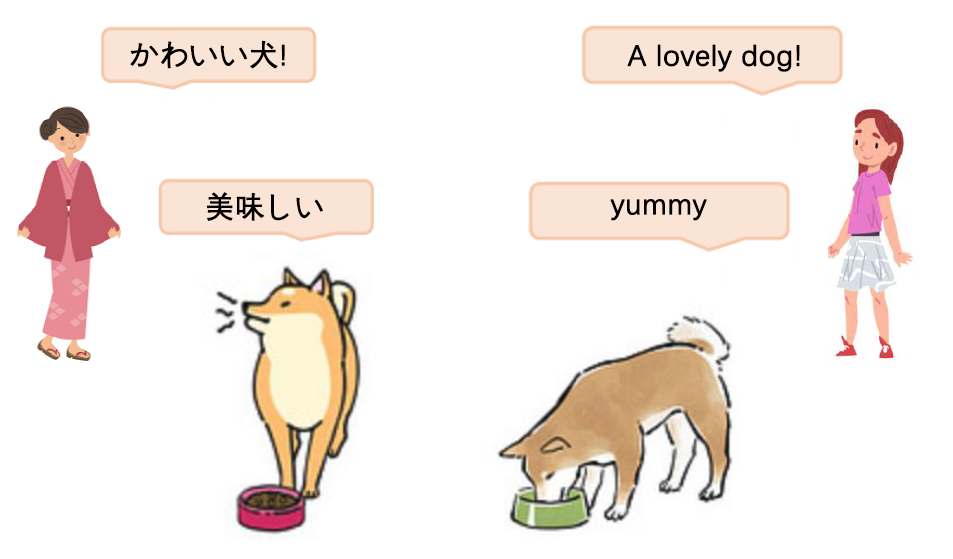
\includegraphics{images/intropic_big_add11.png}}
	\caption{%\KZ{remove the scene tags from the pic.} 
A dog's vocalization may be accousticly correlated with its host language, 
so that a ``Japanese'' dog should vocalize differently than an ``American''
dog under the same context such as ``eating on the lawn''.}
	%\Description {introducing scenario: two shiba inu dogs interact with its hosts in different Japanese and English environment.}
\label{fig:intropic}
\end{figure}

We verify the above hypothesis via a two-stage pipeline. 
First, we conduct classification experiments to investigate the possible
existence of interesting acoustic properties that distinguish dog vocalizations from one language environment to the other. The classification experiment is 
performed on pairs of Japanese and English dog vocal clips under the same \textit{context} which is composed of the \textit{scene category}, \textit{location}, and \textit{activity} of the dog during the recording, so as to exclude  
these confounding non-linguistic factors, which may affect how dogs voice out. 

In stage two, to discover the most prominent factors that distinguish dog vocals 
by their language environments, we perform an importance analysis of different 
factors using Shapley values. A similar analysis is also performed on host 
languages, to study the acoustic difference between English and Japanese. 
Moreover, we compute the Pearson correlation between dog vocals and their host 
speech.  The fact that several most important acoustic characteristics differentiating dogs
have substantial correlations with those of their host language 
(i.e., English or Japanese) supports our hypothesis that 
the domestic dog vocal expressions do share a few acoustic similarities 
with its host language. It is possible that the host language environment has 
an influence over the dog's vocalization. 

Previous dog vocalization datasets are mostly collected under controlled evironment, i.e. the researchers raised several dogs and recorded their physical  as well as vocal behaviours~\cite{ide2021rescue, ehsani2018let, 
molnar2008classification, hantke2018my}. However, such data acquisition methods are not only costly but also lacking generalization capability as the number of dogs is highly restricted. 
%As this method costs a lot and there is no public-released Shiba Inu vocalization dataset, 
Since webly data provides a large amount of dog vocalizations with plenty of metadata featuring the dog breed, language environment and contextual information, we derive a pipeline to obtain and filter the vocals from social media, leading to a large-scale of dog vocalization dataset ``EJShibaVoice''.
The number of families for Japanese and English respectively stand at 219 and 275, much larger than any other similar studies previously reported. 
Moreover, we use the context information tagged with the vocal clips to eliminate the confounding factors in our experiments. 
%To construct the dataset ``EJShibaVoice''
Specifically, we develop 
a framework that crawls Shiba Inu audio clips from both English and 
Japanese-speaking host families, extracts the vocal clips, 
segments the clips into contiguous singular sounds, and tags them with 
contextual information. 


Our main contributions are summarized as follows:

\begin{itemize}
	\item A newly-defined task to uncover the human linguistic influence 
on the vocal expressions of domestic Shiba Inu dogs via a unique data-driven and computational approach, 
which can inspire further research on animal 
languages.~(\secref{sec:assumption}) 
	\item We construct a large-scale Shiba Inu vocalization dataset \textbf{EJShibaVoice} containing clean audio clips produced by dogs from two different language environments: English and Japanese, including dogs' host speech clips. 
The dog vocal and human speech data undergo a systematic pipeline, 
which extracts clean dog voices and the corresponding host speech from 
the social media videos.~(\secref{sec:assumption})
	\item We discover prominent acoustic differences between dogs 
from different language environments: 
	Shiba Inus vocalizations from English-speaking households have a \textbf{\textit{lower frequency}}, 
while those from Japanese environments have \textbf{\textit{faster speed}}, 
which correlates with these two human languages, respectively.~(\secref{sec:main})%by testing several kinds of audio features on our pairwise dataset.
\end{itemize}
